\documentclass[tikz,border=9pt]{standalone}
\usepackage{amsmath,amssymb}
\usetikzlibrary{arrows.meta,positioning,calc}
\begin{document}
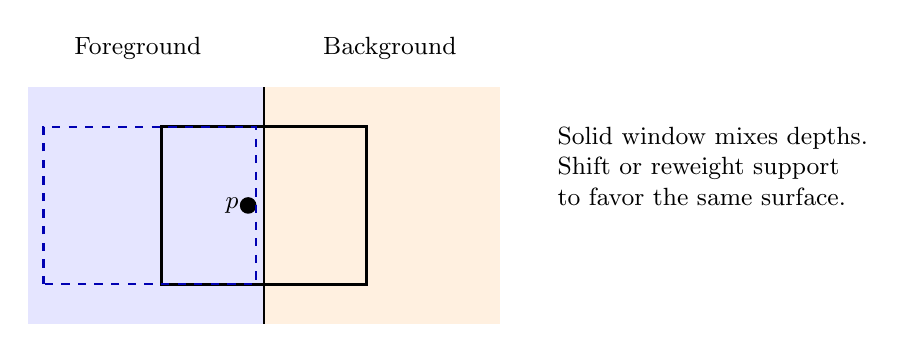
\begin{tikzpicture}[font=\small,arr/.style={-{Stealth},thick},box/.style={draw=blue!55!black,rounded corners,fill=blue!4,align=center,text width=2.9cm,minimum height=1.05cm}]

\fill[blue!10] (0,0) rectangle (3,3);\fill[orange!12] (3,0) rectangle (6,3);
\draw[thick] (3,0)--(3,3);
\node at (1.4,3.5){Foreground};\node at (4.6,3.5){Background};
\draw[very thick] (1.7,.5) rectangle (4.3,2.5);
\fill (2.8,1.5) circle(3pt) node[left]{$p$};
\draw[dashed,thick,blue!70!black] (.2,.5) rectangle (2.9,2.5);
\node[align=left] at (8.7,2){Solid window mixes depths.\\Shift or reweight support\\to favor the same surface.};

\end{tikzpicture}
\end{document}
